% Options for packages loaded elsewhere
\PassOptionsToPackage{unicode}{hyperref}
\PassOptionsToPackage{hyphens}{url}
%
\documentclass[
]{article}
\usepackage{amsmath,amssymb}
\usepackage{lmodern}
\usepackage{iftex}
\ifPDFTeX
  \usepackage[T1]{fontenc}
  \usepackage[utf8]{inputenc}
  \usepackage{textcomp} % provide euro and other symbols
\else % if luatex or xetex
  \usepackage{unicode-math}
  \defaultfontfeatures{Scale=MatchLowercase}
  \defaultfontfeatures[\rmfamily]{Ligatures=TeX,Scale=1}
\fi
% Use upquote if available, for straight quotes in verbatim environments
\IfFileExists{upquote.sty}{\usepackage{upquote}}{}
\IfFileExists{microtype.sty}{% use microtype if available
  \usepackage[]{microtype}
  \UseMicrotypeSet[protrusion]{basicmath} % disable protrusion for tt fonts
}{}
\makeatletter
\@ifundefined{KOMAClassName}{% if non-KOMA class
  \IfFileExists{parskip.sty}{%
    \usepackage{parskip}
  }{% else
    \setlength{\parindent}{0pt}
    \setlength{\parskip}{6pt plus 2pt minus 1pt}}
}{% if KOMA class
  \KOMAoptions{parskip=half}}
\makeatother
\usepackage{xcolor}
\usepackage[margin=1in]{geometry}
\usepackage{graphicx}
\makeatletter
\def\maxwidth{\ifdim\Gin@nat@width>\linewidth\linewidth\else\Gin@nat@width\fi}
\def\maxheight{\ifdim\Gin@nat@height>\textheight\textheight\else\Gin@nat@height\fi}
\makeatother
% Scale images if necessary, so that they will not overflow the page
% margins by default, and it is still possible to overwrite the defaults
% using explicit options in \includegraphics[width, height, ...]{}
\setkeys{Gin}{width=\maxwidth,height=\maxheight,keepaspectratio}
% Set default figure placement to htbp
\makeatletter
\def\fps@figure{htbp}
\makeatother
\setlength{\emergencystretch}{3em} % prevent overfull lines
\providecommand{\tightlist}{%
  \setlength{\itemsep}{0pt}\setlength{\parskip}{0pt}}
\setcounter{secnumdepth}{-\maxdimen} % remove section numbering
\ifLuaTeX
  \usepackage{selnolig}  % disable illegal ligatures
\fi
\IfFileExists{bookmark.sty}{\usepackage{bookmark}}{\usepackage{hyperref}}
\IfFileExists{xurl.sty}{\usepackage{xurl}}{} % add URL line breaks if available
\urlstyle{same} % disable monospaced font for URLs
\hypersetup{
  pdftitle={Experimento 3},
  pdfauthor={Zoe Borrone; Luca Mazzarello; Ignacio Pardo},
  hidelinks,
  pdfcreator={LaTeX via pandoc}}

\title{Experimento 3}
\author{Zoe Borrone \and Luca Mazzarello \and Ignacio Pardo}
\date{2023-08-20}

\begin{document}
\maketitle

source (``exp\_3.R'')

\hypertarget{introducciuxf3n}{%
\subsection{Introducción}\label{introducciuxf3n}}

Para desarrollar este experimento se planteo testear el comportamiento
del modelo al aplicar \emph{One-Hot Enconding} a las variables de los
datasets.

\hypertarget{resultados}{%
\subsection{Resultados}\label{resultados}}

\begin{figure}
\centering
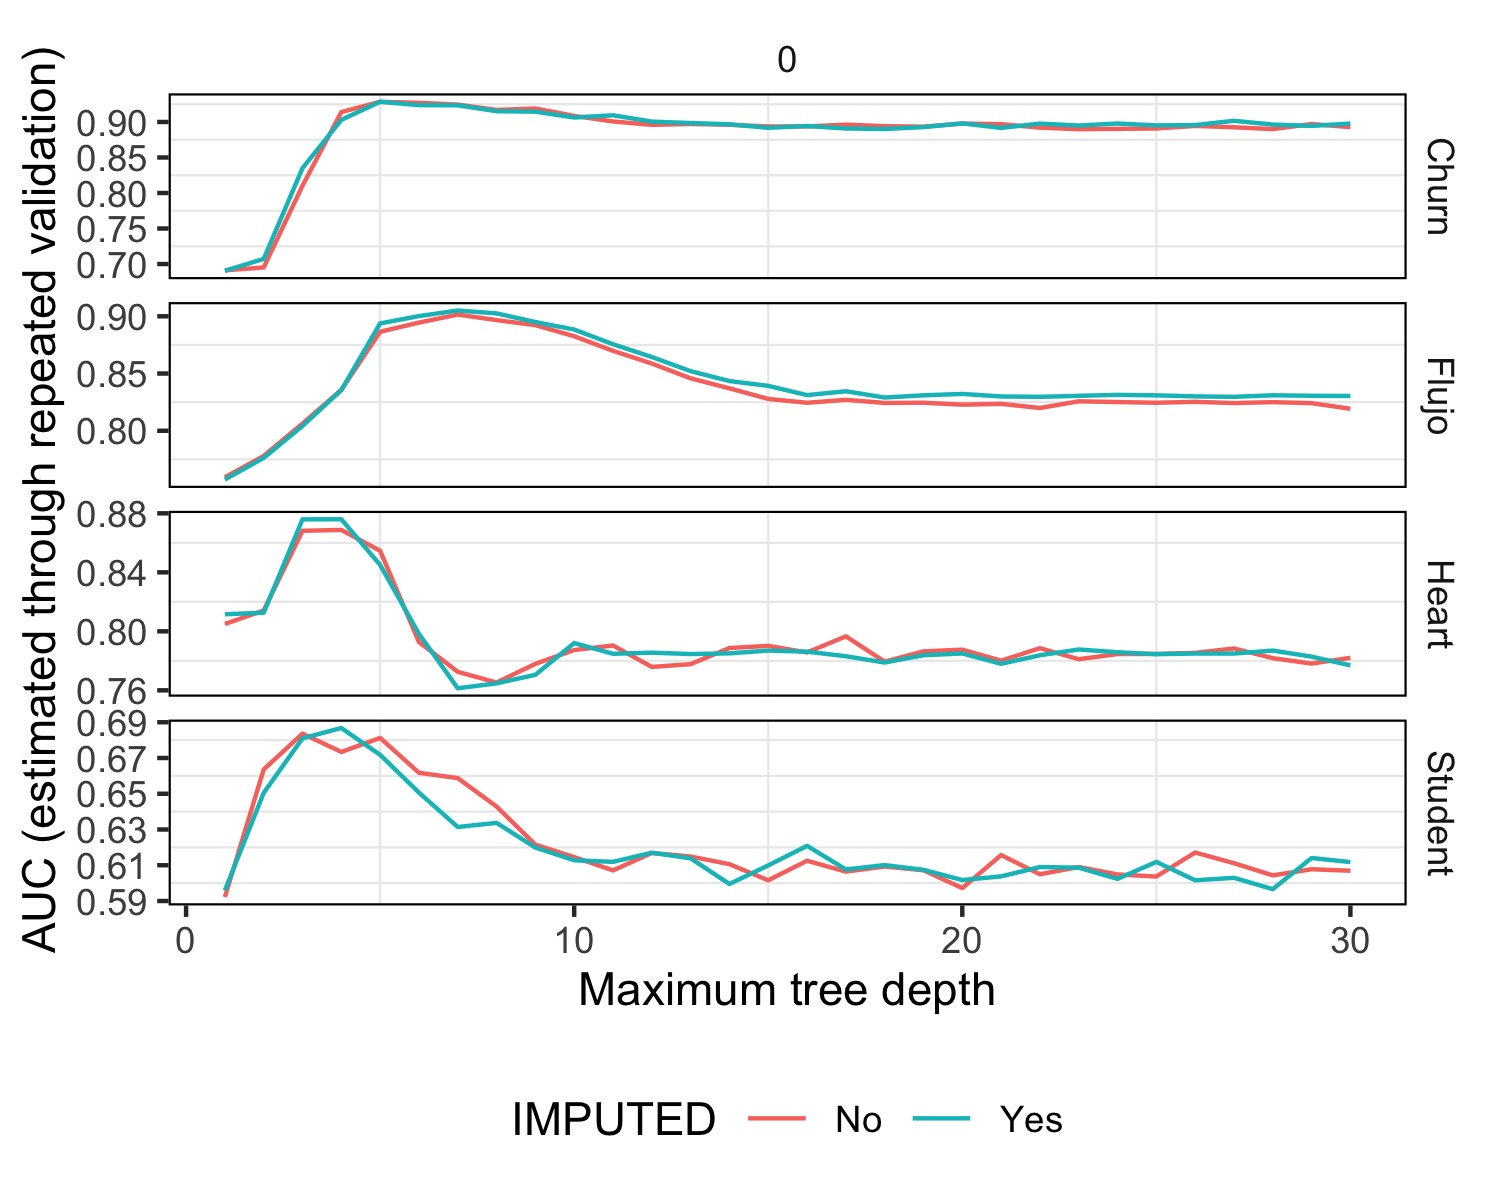
\includegraphics{outputs/plots/exp3.jpg}
\caption{Resultados con y sin One-Hot Enconding}
\end{figure}

En la figura no se logran observar diferencias significativas entre los
resultados obtenidos con y sin \emph{One-Hot Enconding}, por lo que
generamos 3 figuras nuevas una por cada dataset para poder observar
mejor los resultados.

\hypertarget{churn}{%
\subsubsection{Churn}\label{churn}}

Para el dataset de Iranian Churn se observa que el mayor valor de AUC
para el dataset sin \emph{One-Hot Enconding} se obtiene con un maxdepth
de 5, mientras que para el dataset con \emph{One-Hot Enconding} se
obtiene con un maxdepth de 4.

\begin{verbatim}
## # A tibble: 4 x 4
## # Groups:   IMPUTED, ohe [4]
##   maxdepth IMPUTED mean_auc ohe  
##      <int> <chr>      <dbl> <lgl>
## 1        5 Yes        0.932 FALSE
## 2        6 Yes        0.919 TRUE 
## 3        7 No         0.928 FALSE
## 4        8 No         0.920 TRUE
\end{verbatim}

\begin{table}

\caption{\label{tab:unnamed-chunk-2}Churn}
\centering
\begin{tabular}[t]{rlrl}
\toprule
maxdepth & IMPUTED & mean\_auc & ohe\\
\midrule
5 & Yes & 0.9320117 & FALSE\\
6 & Yes & 0.9190171 & TRUE\\
7 & No & 0.9282783 & FALSE\\
8 & No & 0.9196949 & TRUE\\
\bottomrule
\end{tabular}
\end{table}

\includegraphics{exp_3_files/figure-latex/unnamed-chunk-3-1.pdf}

\includegraphics{exp_3_files/figure-latex/unnamed-chunk-4-1.pdf}

\includegraphics{exp_3_files/figure-latex/unnamed-chunk-5-1.pdf}

\end{document}
